\documentclass[a4paper, 11pt, DIV=12, numbers=enddot]{scrartcl}
%\documentclass[a4paper]{article}

%for typing french immediatly into editor
\usepackage[frenchb]{babel}
\usepackage[utf8]{inputenc}
%\usepackage[T1]{fontenc}
\usepackage{lmodern}

\usepackage{graphicx}
\usepackage[ruled] {algorithm}
\usepackage{algpseudocode}
\usepackage{amsfonts,amssymb,amsmath,amsthm}
\usepackage{mathtools}
\usepackage{marvosym}
\usepackage{enumitem}
\usepackage{pgf,tikz}
\usepackage{tikz}
\usepackage{tikz-qtree} 
\usepackage{relsize}
\usepackage{numprint}
\usepackage[position=b]{subcaption}
\usepackage{stmaryrd}
\usetikzlibrary{shapes.geometric}
\usetikzlibrary{arrows}
\usepackage[labelsep = endash]{caption}
\usepackage[colorlinks = false]{hyperref}	
\newcommand\reffig[1]{\hyperref[#1]{\mbox{\figurename~\ref*{#1}}}}
\newcommand\reftbl[1]{\hyperref[#1]{\mbox{\tablename~\ref*{#1}}}}
\newcommand\refanx[1]{\hyperref[#1]{\mbox{\appendixname~\ref*{#1}}}}
\newcommand\cad{c'est-à-dire }
\newcommand\Cad{C'est-à-dire }
%laisse ce commande le \eme par defaut ne marche par chez moi
\newcommand\eme{\textsuperscript{eme}}		
%\pagestyle{empty}
\addto\captionsfrench{\renewcommand{\tablename}{\textsc{Tableau}}}

\addtokomafont{disposition}{\rmfamily}
\renewcommand{\thefootnote}{\alph{footnote}}

\begin{document}
\KOMAoptions{DIV=last}

\newenvironment{claim}[1]{\par\noindent \textbf{Proposition :}\space#1}{}
\newenvironment{claimproof}[1]{\par\noindent \textbf{Preuve :}\space#1}
%{\hfill $\blacksquare$}

% nicer empty set
\let\emptyset\varnothing
% nicer plus sign for inline
\newcommand{\plus}[0]{\text{\raisebox{0.5ex}{\tiny\textbf{+}}}}
\newcommand{\minus}[0]{\text{\raisebox{0.5ex}{\tiny\textbf{-}}}}
\bibliographystyle{plain}

% tikzstuff
\tikzset{
itria/.style={
  draw,dashed,shape border uses incircle,
  isosceles triangle,shape border rotate=90,yshift=-1.45cm},
rtria/.style={
  draw,dashed,shape border uses incircle,
  isosceles triangle,isosceles triangle apex angle=90,
  shape border rotate=-45,yshift=0.2cm,xshift=0.5cm},
ritria/.style={
  draw,dashed,shape border uses incircle,
  isosceles triangle,isosceles triangle apex angle=110,
  shape border rotate=-55,yshift=0.1cm},
letria/.style={
  draw,dashed,shape border uses incircle,
  isosceles triangle,isosceles triangle apex angle=110,
  shape border rotate=235,yshift=0.1cm}
}

\titlehead{	
  \begin{minipage}[c]{1.5cm}
    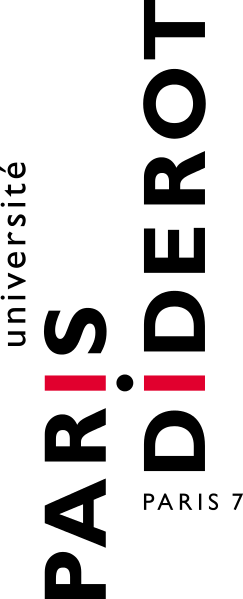
\includegraphics[width=1.5cm]{fig/logo.png}
  \end{minipage} 	
} 	
\title{Izindlela - Projet PFAv}
\author{Lélio Brun et Finn V\"olkel\\
Université Paris Diderot, Paris, France.}
\date{\today}
\maketitle
 
%-----------------------------------------------------------------------
% If your printer does not reproduce dimensions exactly, it may be
% necessary to remove the % signs and adjust the dimensions in the
% following commands:
%
%     \setlength{\textheight}{24cm}
%     \setlength{\textwidth}{16cm}
%
% Similarly for the following, if you need to adjust the positioning
% on the paper:
%
%     \setlength{\topmargin}{-1cm}
%     \setlength{\oddsidemargin}{0pt}
%     \setlength{\evensidemargin}{0pt}
%------------------------------------------------------------------------

\section{Introduction}
\begin{quotation}
\emph{Izindlela} : chemins en Zoulou (d'après Google Traduction).
\end{quotation}

Ce rapport présente notre travail dans le cadre du projet du cours de Programmation Fonctionnelle Avancée.
Nous avons créé en OCaml un petit logiciel de recherche d'itinéraires à partir de données au format OSM (données \emph{OpenStreetMap}).
 
\section{Recherche supportée}

Notre projet implémente 3 types de recherche sur les graphes: Dijkstra, A* avec pour heuristique la distance euclidienne et A* avec pour heuristique la distance euclidienne avec points de repère (\emph{landmarks}, 4 dans notre cas). Nous avons également implémenté un choix de moyen de transport (voiture, vélo ou pièton)  ainsi qu'un choix de critère (rapidité ou distance). Ainsi, les algorithmes tiennent compte des types de routes, des sens uniques ou encore des vitesses maximales autorisées.\newline

De plus, il y a la possibilité de faire la recherche sur un graphe avec des \emph{shortcuts} en perdant l'optimalité du chemin. Par contre la recherche avec les \emph{shortcuts} permet une accélération d'environ 10, principalement grâce au fait que le graphe raccourci est beaucoup plus petit que le graphe normal.\newline

Comme Dijkstra est conçu pour les graphes généraux et ne profite pas du fait que l'on travaille sur un graphe planaire, l'espace de recherche est souvent beaucoup plus grand que celui de A*.

A* euclidien a l'espace de recherche le plus réduit des trois algorithmes.  Ceci est dû au fait que la borne inférieure -- la distance euclidienne -- correspond à l'heuristique \og la plus admissible \fg{} qu'on puisse avoir. A* avec points de repère réduit lui aussi l'espace de recherche par rapport à Dijkstra.\newline 

Néanmoins, malgré des espaces réduits pour les algorithmes de type A*, nous n'avons pas pu remarquer d'amélioration concernant le temps d'exécution. Ceci n'est pas étonnant pour A* euclidien, mais A* avec points de repère est cependant censé apporter une amélioration : le but des points de repères est la \emph{memoization} de l'heuristique, qui évite le calcul de la distance au but pendant la recherche.\newline

Le pré-calcul pour le graphe avec \emph{shortcuts} peut durer longtemps en fonction de la taille de la carte, mais les temps de recherche sont drastiquement accélérés, au détriment de la précision dans le graphe.


\section{Difficultés rencontrées}

Hormis la familiarisation avec \emph{lablgtk} et \emph{lablwebkit}, la programmation en tant que telle ne nous a pas causé de grandes difficultés. \newline

Par contre, le \emph{parsing}, c'est-à-dire la représentation interne des graphes a été plus fastidieuse, en particulier lorsqu'il a fallu implémenter les types de transports ou les critères (rapidité ou distance). En effet, déméler les \emph{tags} OSM n'est pas aisé, pas plus que la vérification, qui implique une visualisation adéquate (type de route empruntée, sens unique, etc.). De plus, les données étant potentiellement très fournies, il a fallu porter une attention particulière à nos fonctions de \emph{parsing} récursives, de façon à éviter les \emph{stack overflows}.

Ainsi, par exemple, notre projet initial de proposer un A* avec une heuristique permettant de choisir le chemin le plus sympathique pour un cycliste a été avorté. \newline

Cependant, nos plus gros problèmes ont été rencontrés sur l'implémentation même des algorithmes. Il est à noter que les améliorations que nous estimons nécessaires vont pour la plupart en ce sens. En effet, il est possible de trouver des erreurs de comportement, par exemple concernant la reconstruction du chemin emprunté ou la perte d'optimalité inattendue de certains itinéraires.

\newpage
\section{Remarques}

L'interface graphique d'Izindlela repose sur \emph{lablgtk} et notamment sur \emph{lablwebkit} pour la visualisation : en effet nous avons estimé que profiter des API Web pour \emph{OpenStreetMap} (MapBox, Leafleft) était le moyen le plus simple et le plus rapide d'obtenir une visualisation efficace.

Ainsi, l'application fait appel à un petit peu de code HTML et de Javascript, ce qui sors du cadre de ce cours, mais nous nous sommes contraints à réduire ces parties de code au minimum. Nous avons remarqué que cette solution semble se comporter différemment selon les machines (bugs d'affichage de l'itinéraire), soulignant un manque de robusteese.

\section{Aperçu}
Les figures suivantes permettent d'apprécier les différences en terme d'espace de recherche et de temps de calcul entre les différents algorithmes implémentés.\newline

On constate que les A* explorent beaucoup moins de n\oe uds que Dijkstra qui étend sa recherche de manière uniforme (et donc circulaire). Contrairement à ce qui était attendu, les points de repères ne permettent pas de gain en terme de temps de calcul.

Enfin, on remarque bien que les espaces de recherche des versions \og raccourcies \fg{} explorent un espace bien moins dense, ce qui réduit considérablement le temps de recherche.\newline

La carte ici étant très étendue, on obtient pour les versions normales des algorithmes des temps de calcul relativement élevés, même pour un parcours qui n'excède pas les 5km. Sur une carte plus réduite, ces temps sont réduits en conséquence.

\begin{figure}[!h]
  \centering
  \begin{subfigure}[b]{.49\textwidth}
    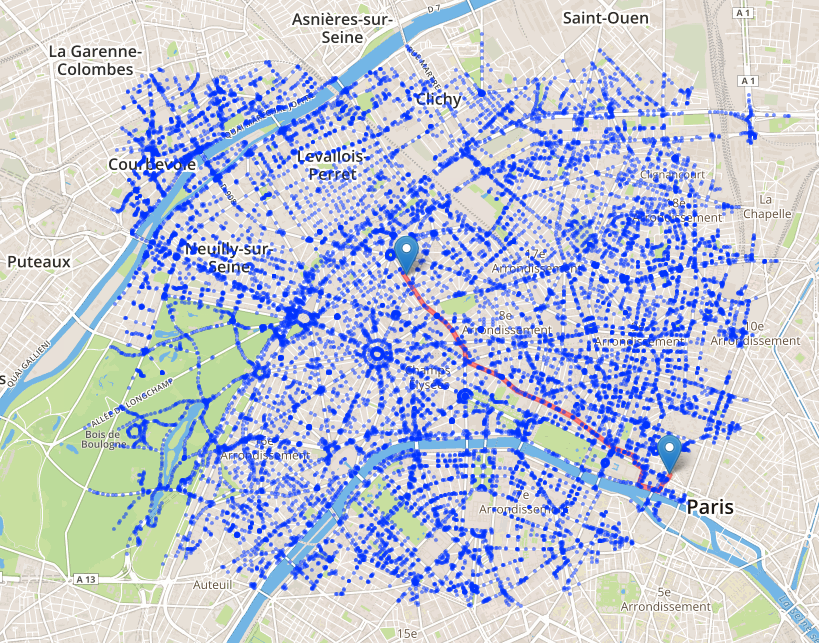
\includegraphics[width=\textwidth]{fig/dijkstra.png}
    \caption{Dijkstra normal - \numprint[s]{2.266}}
  \end{subfigure}
  \hfill
  \begin{subfigure}[b]{.49\textwidth}
    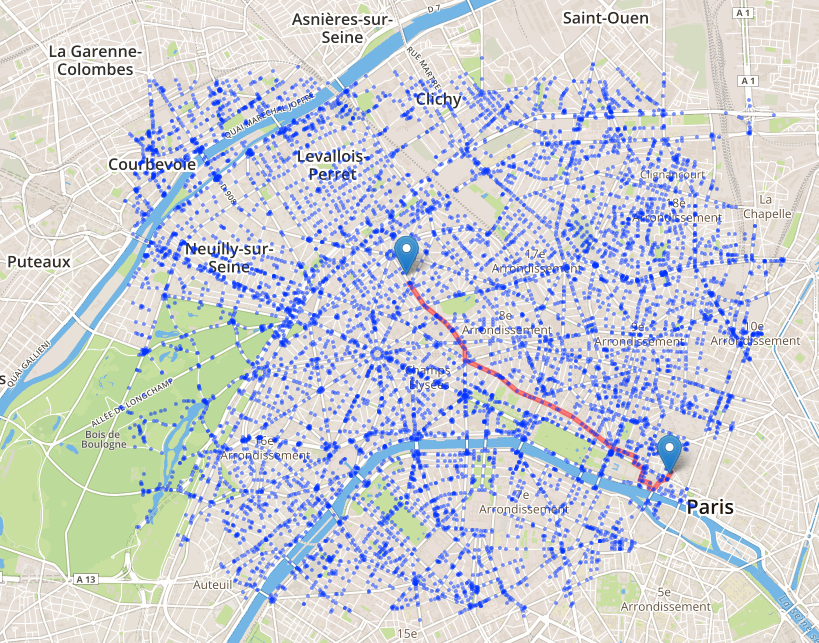
\includegraphics[width=\textwidth]{fig/dijkstra_hl.png}
    \caption{Dijkstra \emph{shortcuts} - \numprint[s]{0.057}}
  \end{subfigure}
  \newline\newline
  \begin{subfigure}[b]{.49\textwidth}
    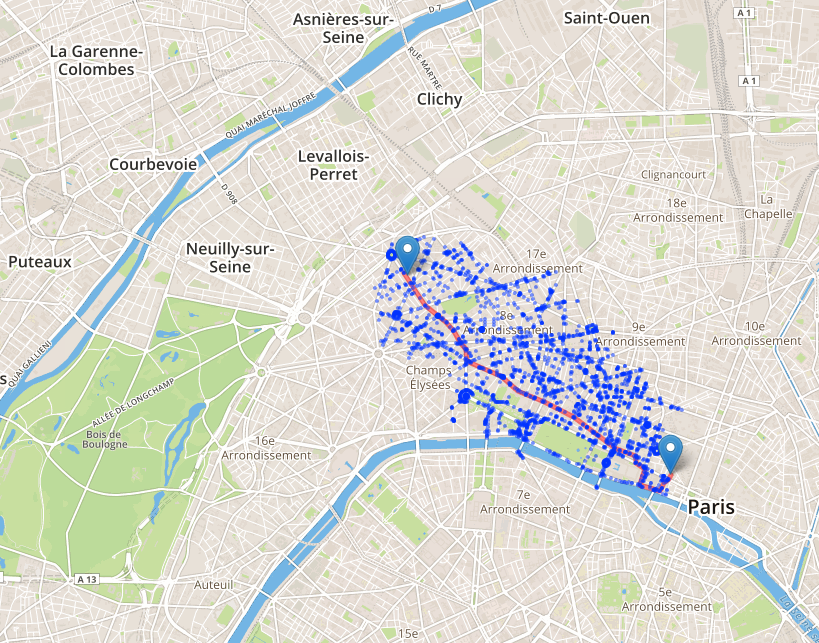
\includegraphics[width=\textwidth]{fig/euclidien.png}
    \caption{A* euclidien normal - \numprint[s]{2.088}}
  \end{subfigure}
  \hfill
  \begin{subfigure}[b]{.49\textwidth}
    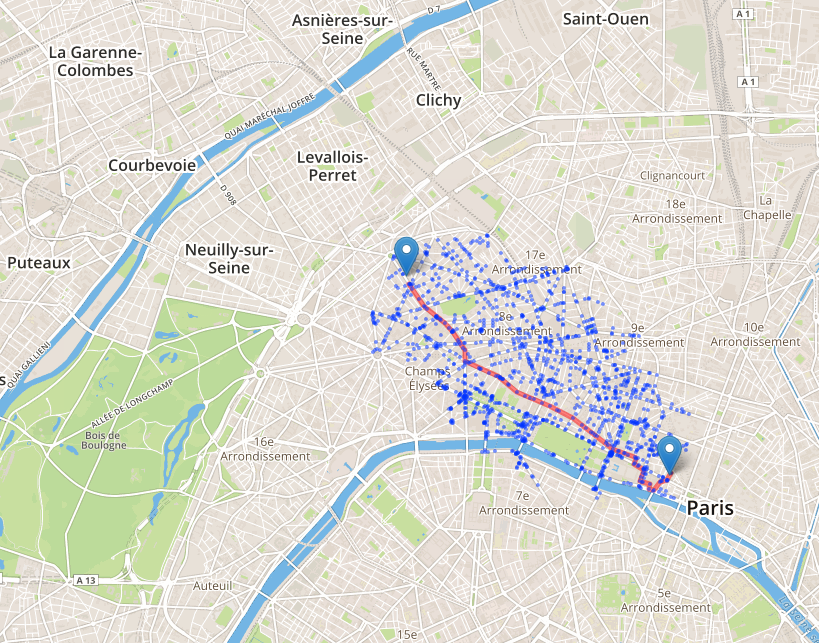
\includegraphics[width=\textwidth]{fig/euclidien_hl.png}
    \caption{A* euclidien \emph{shortcuts} - \numprint[s]{0.035}}
  \end{subfigure}
  \newline\newline
  \begin{subfigure}[b]{.49\textwidth}
    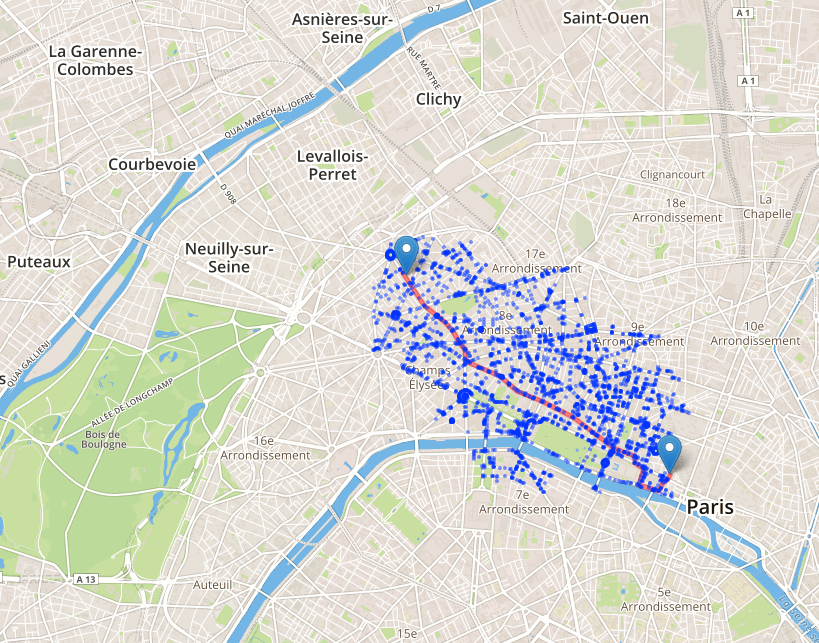
\includegraphics[width=\textwidth]{fig/landmarks.png}
    \caption{A* \emph{landmarks} normal - \numprint[s]{2.116}}
  \end{subfigure}
  \hfill
  \begin{subfigure}[b]{.49\textwidth}
    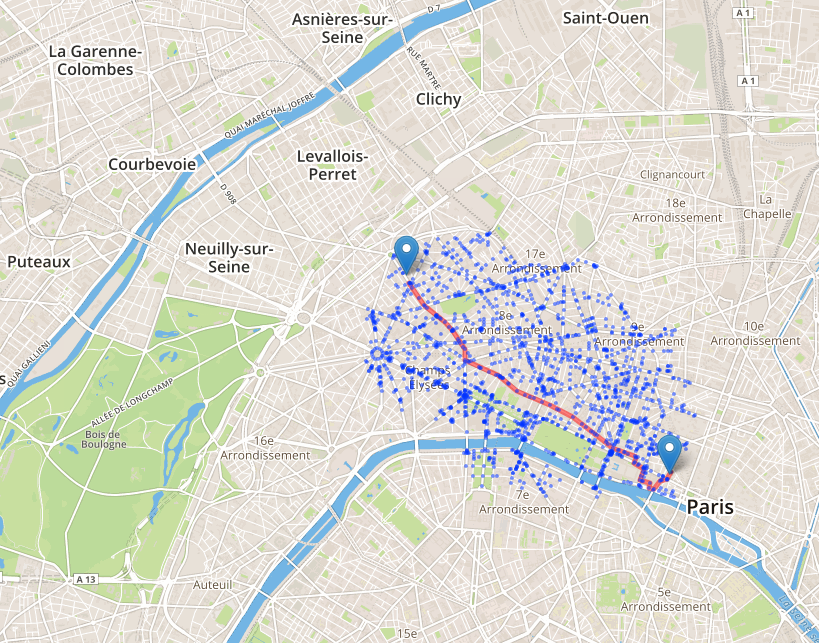
\includegraphics[width=\textwidth]{fig/landmarks_hl.png}
    \caption{A* \emph{landmarks} \emph{shortcuts} - \numprint[s]{0.039}}
  \end{subfigure}
  %\caption{A* points de repères}
\end{figure}

\end{document}
